%%%%%%%%%%%%%%%%%%%%%%%%%%%%%%%%%%%%%%%%%%%%%%
%                insertmeeting
% 1) Title (something creative & funny?)
% 2) Date (MM/DD/YYYY)
% 3) Location (ex. Hagerty High School)
% 4) People/Committees Present 
% 5) Picture 
% 6) Start Time & Stop Time (ex. 12:30AM to 4:30PM)
%%%%%%%%%%%%%%%%%%%%%%%%%%%%%%%%%%%%%%%%%%%%%%
\insertmeeting 
	{Intake Invention} 
	{08/20/21}
	{Hagerty High School}
	{Nathan, also talked to Jensen and Ritam outside of the meeting}
	{Images/RobotPics/robot.jpg}
	{6:00 - 8:00}
	
\subsection*{Hardware}
\noindent\hfil\rule{\textwidth}{.4pt}\hfil
\subsubsection*{Goals}
\begin{itemize}
    \item Design prototype for intake

\end{itemize} 

\noindent\hfil\rule{\textwidth}{.4pt}\hfil

\subsubsection*{Accomplishments}
Now that we’ve built the rev hub holder and while we are waiting for the churros to be threaded, we wanted to start something new. One of the few things that we know about the upcoming seasons is two of the game elements that we will be using. They are wiffle balls and cubes (image 1) These game elements have been used in the past, which means that we have some examples to take inspiration from, however, we still want to test all of the designs on our own. One of the main types of intakes used in the rover ruckus season utilizes a sweeper with surgical tubing that pushes the balls and cubes into the robot (image 2- credit: team 6929 data force).The other main type was one that 4717 used in the past and is more common in vex competitions. This second design uses rubber bands stretched between 2 disks or sprockets that spins and sucks in the game elements (image 3). We think that one of these 2 designs could be a future design on our robot so we plan to test both. One thing that we think will be important for this test will be that the sweeper and rubber band sub-assemblies be interchangeable while keeping the frame, structure, and motors the same so we know outside factors aren’t affecting the two options differently.
With our newly found inspiration, we started sketching designs (image 4). We started off thinking of using a coaxial mechanism similar to what we used in the Ultimate Goal season, but found that it would be less space efficient and more susceptible to structural failure. Although these factors wouldn’t affect the testing of the designs very much, as we aren't actually planning on attaching them to the robot yet, we came up with a new idea we want to try out. Instead of having an arm that pivots like on the coaxial design, our idea is to have a slot that an axel can rest in but that allows it to slide upwards if a game element goes through it. Although both the coaxial and slot designs allow the intake to adapt to different size elements, the slot design should be more space efficient and stronger. The only downside to the design is that we aren't sure if it will work, so we will test it along with the rubber band and sweeper designs. One other important aspect of our plan, is that we will have the drive great be larger than the follower gear to gear down the intake so it spins faster. This is important because we are planning on using vex motors, which don’t spin as fast as we want them to for this intake.
Once we came up with our design, we started creating it in CAD. To ensure that we could easily change important dimensions later, we started with a skeleton. This includes all of the important dimensions and is the basis of the whole design (image 5). After creating the skeleton, we made the side plates, taking many of its dimensions from the skeleton, but adding a form around the design. From there we created a bottom plate and a tie plate to hold the two sides together. Learning from our mistake with the rev hub holder, we added lots of t-slot joints to ensure all of the sides are held firmly together. Then, we realized a flaw in our design. At its current height, the vex motor we wanted to use would be in the way of the back of the intake. Although this wasn’t a major problem and the intake would still work, allowing game elements to pass all the way through would make it easier to test the speed of the intake in picking up more than 2 cubes or balls. Because we made the skeleton at the beginning, we were able to change the motor position by about .25 inches, and due to the parametric nature of how we sketched it, other parts of the design dependent on the motor position, like the slot location, changed automatically. This shows how important skeletons can be if we decide to make corrections later on. After correcting our error, we added holes to the plates to reduce their weight and created an assembly where we added all of the plates, as well as vex sprockets, motors, and bearing blocks that we downloaded from their website (image 6).
After creating the assembly for the intake structure, we needed to create designs for the sweeper and rubber band spinners. It was important that they be interchangeable, so we can test them using the same main structure. The way that we decided to do this was to make the central axle slide out from both mechanisms so we can slide one off and the other on. We started designing the sweeper intake first, modeling the size pvc pipe we plan to use, then creating 3d printable caps that will slide into the end of the pipe. Although the caps were the only part of the sweeper that needed to be modeled, we also added the surgical tubing and pvc pipe to get a better feel for the design (image 7). Next we started designing the rubber band part of the intake. We sketched some 3d printable hubs and a notched disk we intend to laser cut that will hold the rubber bands in place (image 8). 
We inserted all of the parts from both intakes, however, we still needed to create a new configuration that would allow us to switch between the sweeper and rubber band designs easily. Although we could have created 2 different assemblies for the 2 different designs, using 2 assemblies would make it more difficult to make changes in other parts of the assembly. We created our configurations for each of the designs, supressign the unneeded intake parts for each configuration (image 9). With the configurations created, we could now easily switch between the 2 designs, just like we will be able to when we build the intake (image 10)

\begin{figure}[ht]
\centering
\begin{minipage}[b]{.50\textwidth}
  \centering
  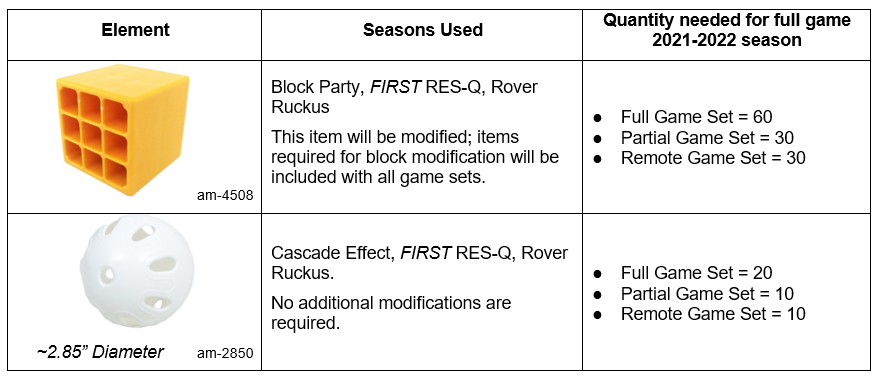
\includegraphics[width=0.8\textwidth]{Meetings/August/08-20-21/8-18-21_CAD_Image1 - Nathan Forrer.png}
  \caption{Whiffle balls and cubes are being used as this year's game elements.}
  \label{fig:pic1}
\end{minipage}%
\hfill%
\begin{minipage}[b]{.50\textwidth}
  \centering
  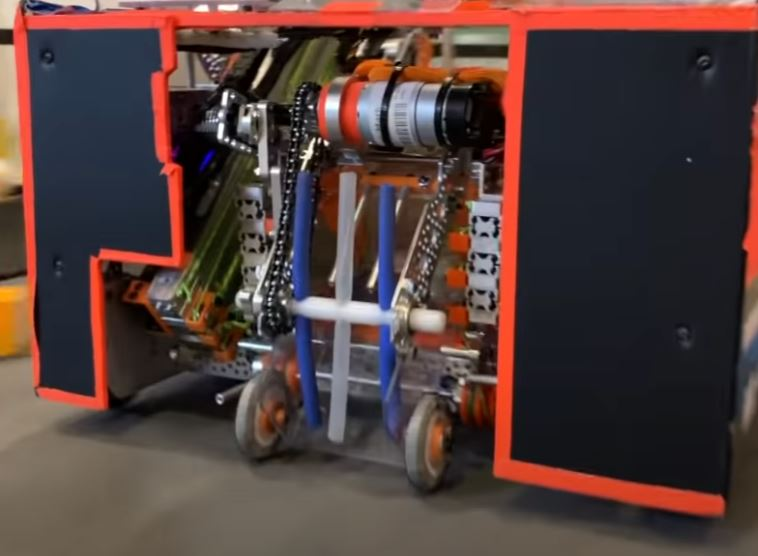
\includegraphics[width=0.8\textwidth]{Meetings/August/08-20-21/8-18-21_CAD_Image2 - Nathan Forrer.jpg}
  \caption{An example sweeper from FTC 6929 Data Force. We plan to implement a simiar mechanism.}
  \label{fig:pic2}
\end{minipage}
\end{figure}

\begin{figure}[ht]
\centering
\begin{minipage}[b]{.50\textwidth}
  \centering
  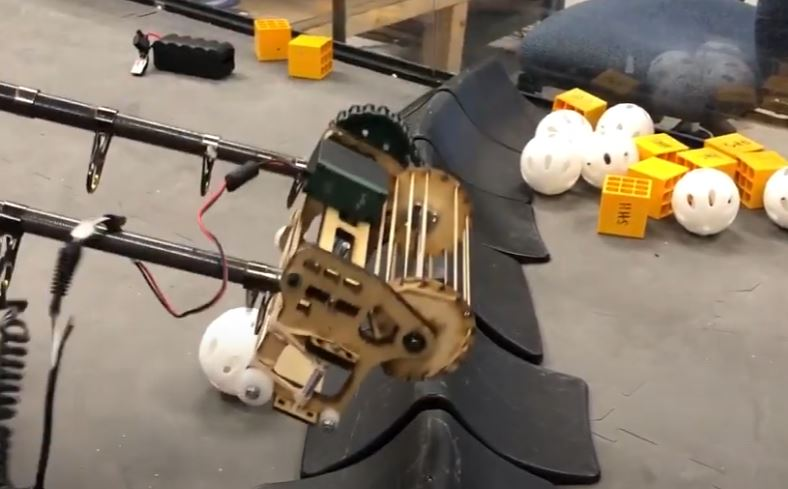
\includegraphics[width=0.8\textwidth]{Meetings/August/08-20-21/8-18-21_CAD_Image3 - Nathan Forrer.jpg}
  \caption{A second design for an intake that our sister team, FTC 4227, used in Rover Ruckus}
  \label{fig:pic3}
\end{minipage}%
\hfill%
\begin{minipage}[b]{.50\textwidth}
  \centering
  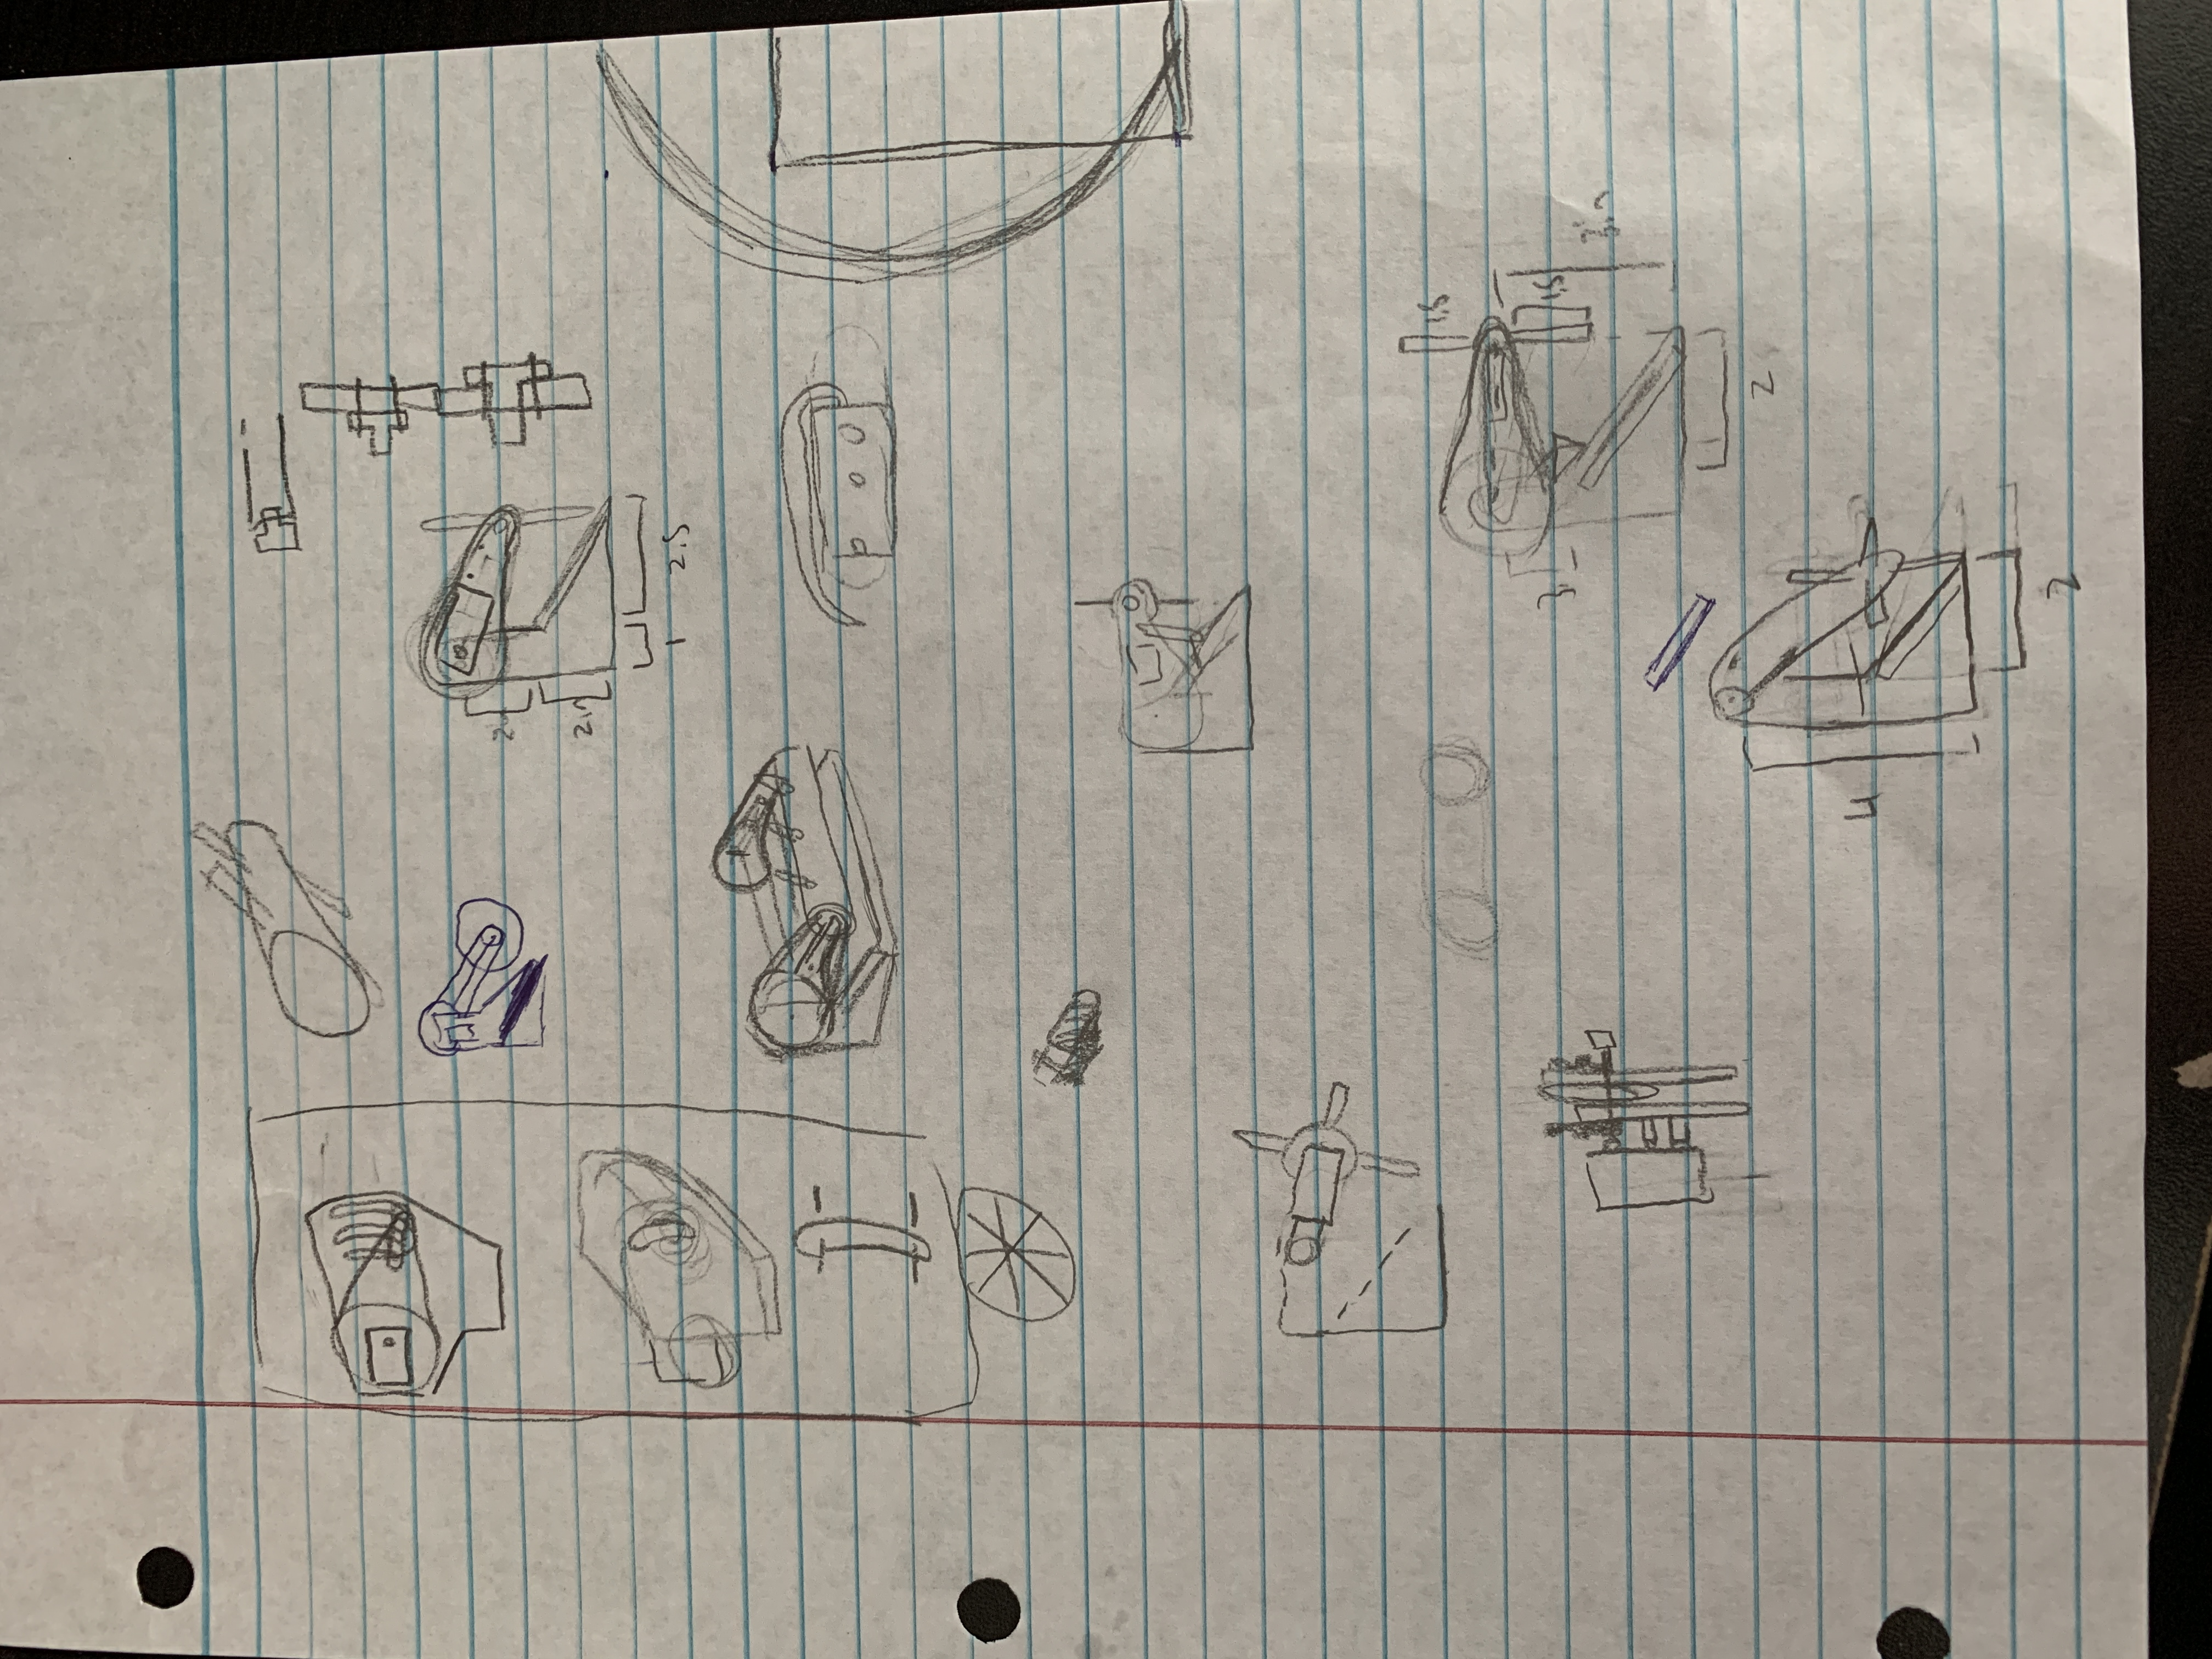
\includegraphics[width=0.8\textwidth]{Meetings/August/08-20-21/8-18-21_CAD_Image4 - Nathan Forrer.jpg}
  \caption{Our "brainstorming sheet" for intakes.}
  \label{fig:pic4}
\end{minipage}
\end{figure}

\begin{figure}[ht]
\centering
\begin{minipage}[b]{.50\textwidth}
  \centering
  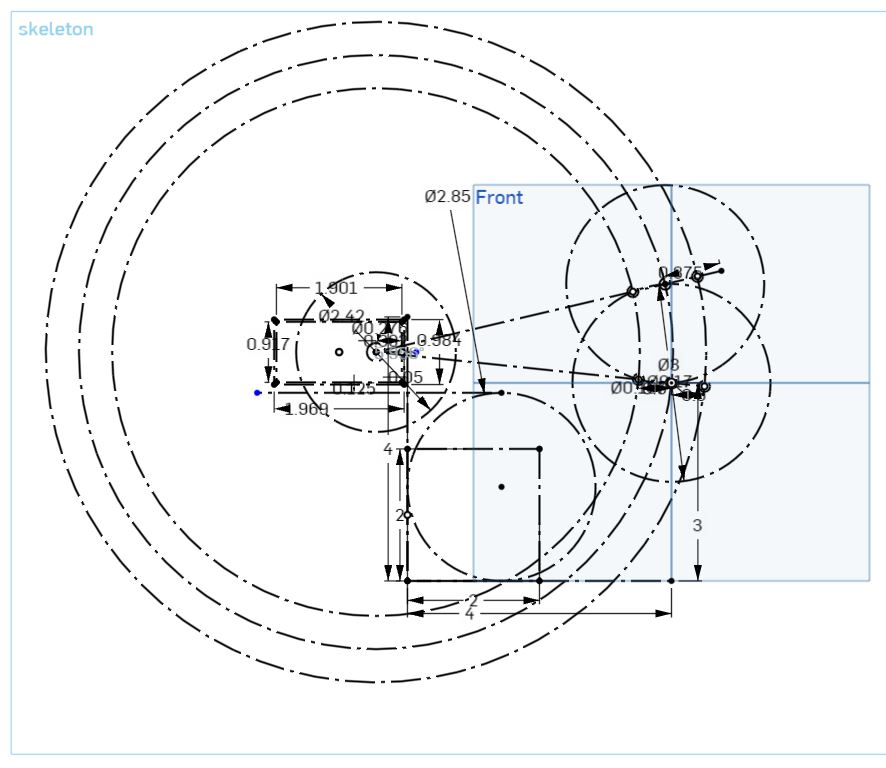
\includegraphics[width=0.8\textwidth]{Meetings/August/08-20-21/8-18-21_CAD_Image5 - Nathan Forrer.jpg}
  \caption{This is our skeleton for an intake design}
  \label{fig:pic5}
\end{minipage}%
\hfill%
\begin{minipage}[b]{.50\textwidth}
  \centering
  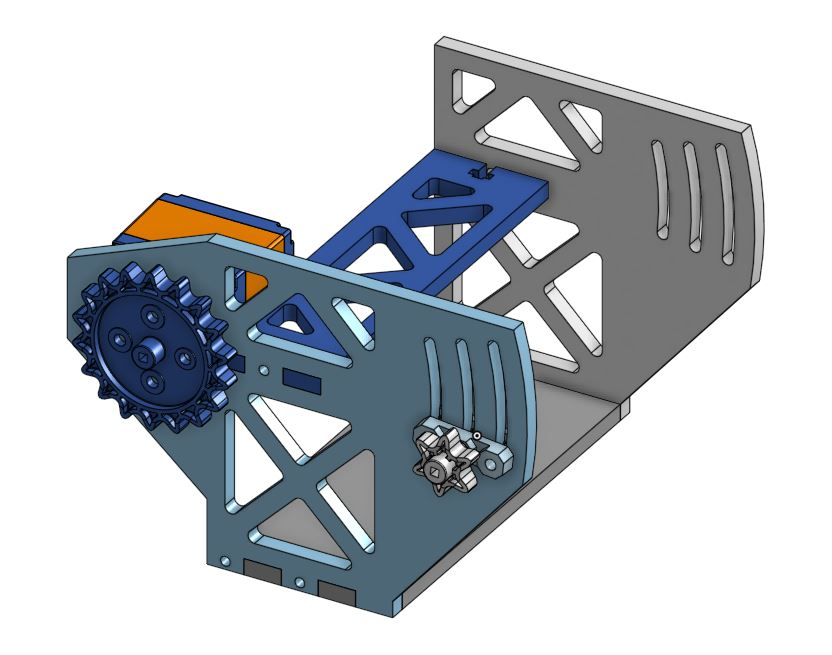
\includegraphics[width=0.8\textwidth]{Meetings/August/08-20-21/8-18-21_CAD_Image6 - Nathan Forrer.jpg}
  \caption{Our first design for the intake following the skeleton shown in Figure 5}
  \label{fig:pic6}
\end{minipage}
\end{figure}

\begin{figure}[ht]
\centering
\begin{minipage}[b]{.50\textwidth}
  \centering
  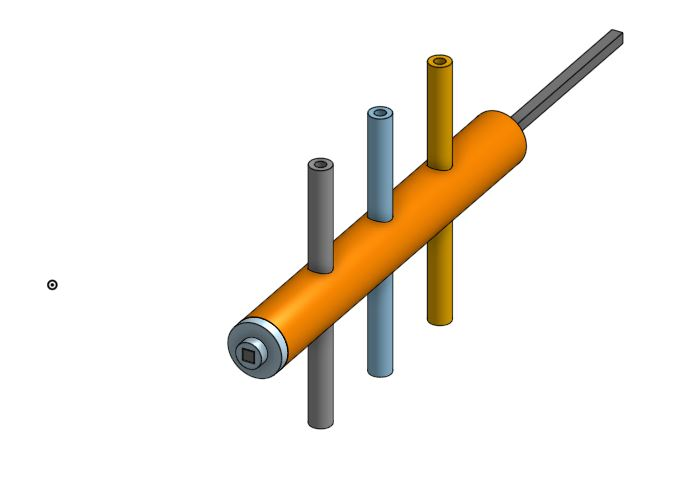
\includegraphics[width=0.8\textwidth]{Meetings/August/08-20-21/8-18-21_CAD_Image7 - Nathan Forrer.jpg}
  \caption{Basing our design on some examples from other teams, we plan to implement a similar sweeper using rubber tubes.}
  \label{fig:pic7}
\end{minipage}%
\hfill%
\begin{minipage}[b]{.50\textwidth}
  \centering
  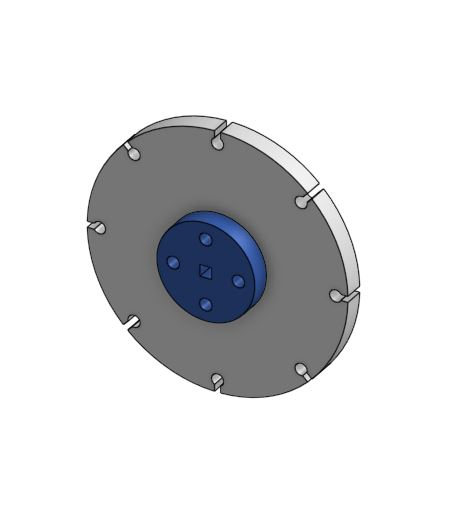
\includegraphics[width=0.8\textwidth]{Meetings/August/08-20-21/8-18-21_CAD_Image8 - Nathan Forrer.jpg}
  \caption{The custom hub we created to hold the rubber bands.}
  \label{fig:pic8}
\end{minipage}
\end{figure}

\begin{figure}[ht]
\centering
\begin{minipage}[b]{.50\textwidth}
  \centering
  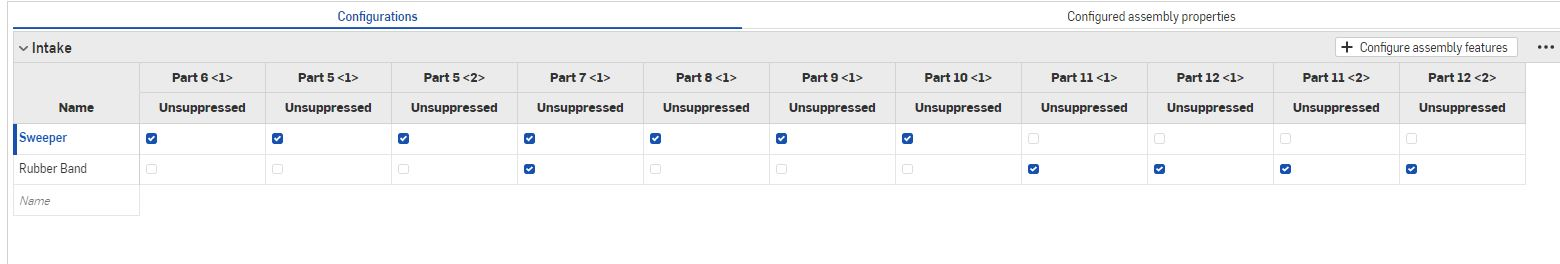
\includegraphics[width=0.8\textwidth]{Meetings/August/08-20-21/8-18-21_CAD_Image9 - Nathan Forrer.jpg}
  \caption{Our suppressions for the different parts of the assembly.}
  \label{fig:pic9}
\end{minipage}%
\hfill%
\begin{minipage}[b]{.50\textwidth}
  \centering
  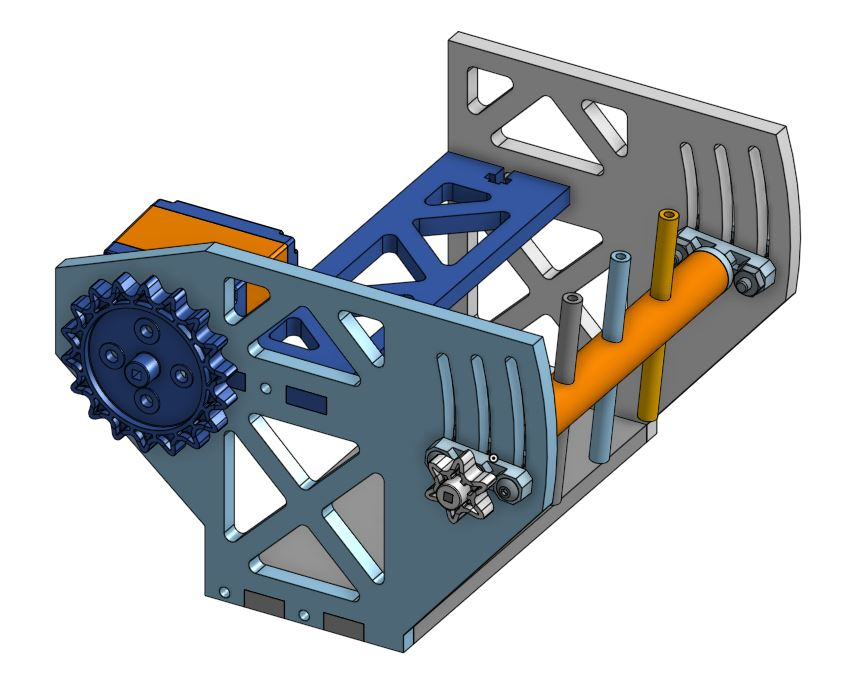
\includegraphics[width=0.8\textwidth]{Meetings/August/08-20-21/8-18-21_CAD_Image10 - Nathan Forrer.jpg}
  \caption{The current state of our intake.}
  \label{fig:pic10}
\end{minipage}
\end{figure}